% Options for packages loaded elsewhere
\PassOptionsToPackage{unicode}{hyperref}
\PassOptionsToPackage{hyphens}{url}
%
\documentclass[
]{book}
\usepackage{amsmath,amssymb}
\usepackage{iftex}
\ifPDFTeX
  \usepackage[T1]{fontenc}
  \usepackage[utf8]{inputenc}
  \usepackage{textcomp} % provide euro and other symbols
\else % if luatex or xetex
  \usepackage{unicode-math} % this also loads fontspec
  \defaultfontfeatures{Scale=MatchLowercase}
  \defaultfontfeatures[\rmfamily]{Ligatures=TeX,Scale=1}
\fi
\usepackage{lmodern}
\ifPDFTeX\else
  % xetex/luatex font selection
\fi
% Use upquote if available, for straight quotes in verbatim environments
\IfFileExists{upquote.sty}{\usepackage{upquote}}{}
\IfFileExists{microtype.sty}{% use microtype if available
  \usepackage[]{microtype}
  \UseMicrotypeSet[protrusion]{basicmath} % disable protrusion for tt fonts
}{}
\makeatletter
\@ifundefined{KOMAClassName}{% if non-KOMA class
  \IfFileExists{parskip.sty}{%
    \usepackage{parskip}
  }{% else
    \setlength{\parindent}{0pt}
    \setlength{\parskip}{6pt plus 2pt minus 1pt}}
}{% if KOMA class
  \KOMAoptions{parskip=half}}
\makeatother
\usepackage{xcolor}
\usepackage{color}
\usepackage{fancyvrb}
\newcommand{\VerbBar}{|}
\newcommand{\VERB}{\Verb[commandchars=\\\{\}]}
\DefineVerbatimEnvironment{Highlighting}{Verbatim}{commandchars=\\\{\}}
% Add ',fontsize=\small' for more characters per line
\usepackage{framed}
\definecolor{shadecolor}{RGB}{248,248,248}
\newenvironment{Shaded}{\begin{snugshade}}{\end{snugshade}}
\newcommand{\AlertTok}[1]{\textcolor[rgb]{0.94,0.16,0.16}{#1}}
\newcommand{\AnnotationTok}[1]{\textcolor[rgb]{0.56,0.35,0.01}{\textbf{\textit{#1}}}}
\newcommand{\AttributeTok}[1]{\textcolor[rgb]{0.13,0.29,0.53}{#1}}
\newcommand{\BaseNTok}[1]{\textcolor[rgb]{0.00,0.00,0.81}{#1}}
\newcommand{\BuiltInTok}[1]{#1}
\newcommand{\CharTok}[1]{\textcolor[rgb]{0.31,0.60,0.02}{#1}}
\newcommand{\CommentTok}[1]{\textcolor[rgb]{0.56,0.35,0.01}{\textit{#1}}}
\newcommand{\CommentVarTok}[1]{\textcolor[rgb]{0.56,0.35,0.01}{\textbf{\textit{#1}}}}
\newcommand{\ConstantTok}[1]{\textcolor[rgb]{0.56,0.35,0.01}{#1}}
\newcommand{\ControlFlowTok}[1]{\textcolor[rgb]{0.13,0.29,0.53}{\textbf{#1}}}
\newcommand{\DataTypeTok}[1]{\textcolor[rgb]{0.13,0.29,0.53}{#1}}
\newcommand{\DecValTok}[1]{\textcolor[rgb]{0.00,0.00,0.81}{#1}}
\newcommand{\DocumentationTok}[1]{\textcolor[rgb]{0.56,0.35,0.01}{\textbf{\textit{#1}}}}
\newcommand{\ErrorTok}[1]{\textcolor[rgb]{0.64,0.00,0.00}{\textbf{#1}}}
\newcommand{\ExtensionTok}[1]{#1}
\newcommand{\FloatTok}[1]{\textcolor[rgb]{0.00,0.00,0.81}{#1}}
\newcommand{\FunctionTok}[1]{\textcolor[rgb]{0.13,0.29,0.53}{\textbf{#1}}}
\newcommand{\ImportTok}[1]{#1}
\newcommand{\InformationTok}[1]{\textcolor[rgb]{0.56,0.35,0.01}{\textbf{\textit{#1}}}}
\newcommand{\KeywordTok}[1]{\textcolor[rgb]{0.13,0.29,0.53}{\textbf{#1}}}
\newcommand{\NormalTok}[1]{#1}
\newcommand{\OperatorTok}[1]{\textcolor[rgb]{0.81,0.36,0.00}{\textbf{#1}}}
\newcommand{\OtherTok}[1]{\textcolor[rgb]{0.56,0.35,0.01}{#1}}
\newcommand{\PreprocessorTok}[1]{\textcolor[rgb]{0.56,0.35,0.01}{\textit{#1}}}
\newcommand{\RegionMarkerTok}[1]{#1}
\newcommand{\SpecialCharTok}[1]{\textcolor[rgb]{0.81,0.36,0.00}{\textbf{#1}}}
\newcommand{\SpecialStringTok}[1]{\textcolor[rgb]{0.31,0.60,0.02}{#1}}
\newcommand{\StringTok}[1]{\textcolor[rgb]{0.31,0.60,0.02}{#1}}
\newcommand{\VariableTok}[1]{\textcolor[rgb]{0.00,0.00,0.00}{#1}}
\newcommand{\VerbatimStringTok}[1]{\textcolor[rgb]{0.31,0.60,0.02}{#1}}
\newcommand{\WarningTok}[1]{\textcolor[rgb]{0.56,0.35,0.01}{\textbf{\textit{#1}}}}
\usepackage{longtable,booktabs,array}
\usepackage{calc} % for calculating minipage widths
% Correct order of tables after \paragraph or \subparagraph
\usepackage{etoolbox}
\makeatletter
\patchcmd\longtable{\par}{\if@noskipsec\mbox{}\fi\par}{}{}
\makeatother
% Allow footnotes in longtable head/foot
\IfFileExists{footnotehyper.sty}{\usepackage{footnotehyper}}{\usepackage{footnote}}
\makesavenoteenv{longtable}
\usepackage{graphicx}
\makeatletter
\def\maxwidth{\ifdim\Gin@nat@width>\linewidth\linewidth\else\Gin@nat@width\fi}
\def\maxheight{\ifdim\Gin@nat@height>\textheight\textheight\else\Gin@nat@height\fi}
\makeatother
% Scale images if necessary, so that they will not overflow the page
% margins by default, and it is still possible to overwrite the defaults
% using explicit options in \includegraphics[width, height, ...]{}
\setkeys{Gin}{width=\maxwidth,height=\maxheight,keepaspectratio}
% Set default figure placement to htbp
\makeatletter
\def\fps@figure{htbp}
\makeatother
\setlength{\emergencystretch}{3em} % prevent overfull lines
\providecommand{\tightlist}{%
  \setlength{\itemsep}{0pt}\setlength{\parskip}{0pt}}
\setcounter{secnumdepth}{5}
\usepackage{booktabs}
\ifLuaTeX
  \usepackage{selnolig}  % disable illegal ligatures
\fi
\usepackage[]{natbib}
\bibliographystyle{plainnat}
\usepackage{bookmark}
\IfFileExists{xurl.sty}{\usepackage{xurl}}{} % add URL line breaks if available
\urlstyle{same}
\hypersetup{
  pdftitle={WildlifeSystems - biodiversity technologies},
  pdfauthor={Ed Baker},
  hidelinks,
  pdfcreator={LaTeX via pandoc}}

\title{WildlifeSystems - biodiversity technologies}
\author{\href{https://ebaker.me.uk}{Ed Baker}}
\date{2024-11-17}

\begin{document}
\maketitle

{
\setcounter{tocdepth}{1}
\tableofcontents
}
\chapter*{About}\label{about}
\addcontentsline{toc}{chapter}{About}

This book explains the technologies developed as part of \href{https://wildlife.systems}{WildlifeSystems} and how they can be implemented in real-world scenarios.

\section*{Support}\label{support}
\addcontentsline{toc}{section}{Support}

WildlifeSystems nodes were originally developed and used as part of the Leverhulme Trust funded \href{https://ebaker.me.uk/aao}{Automated Acoustic Observatories} project at the University of York. Additional development is undertaken as part of the \href{https://www.nhm.ac.uk/about-us/urban-nature-project.html}{Urban Nature Project} at the Natural History Museum, London.

\chapter{Biodiversity Technologies}\label{biodiversity-technologies}

\section{What are Biodiversity Technologies?}\label{what-are-biodiversity-technologies}

Biodiversity technologies are tools that allow researchers and others to study, monitor and
conserve biodiversity. These tools can be used to monitor a wide range of species, habitats, and ecosystems, potentially in (near) real-time and/or from a great distance away.

\subsection{What has enabled Biodiversity Technologies?}\label{what-has-enabled-biodiversity-technologies}

The development of biodiversity technologies has been enabled by the rapid advances in sensor technology, data processing, and communication networks. These technologies have made it possible to collect, store, and analyse large amounts of data from a wide range of sources, including remote sensors, cameras, and acoustic recorders.

This has been accompanied by a decline in the cost of these technologies (e.g.~Figure \ref{fig:storage-costs}), making them more accessible to researchers, conservationists, and others interested in monitoring biodiversity.

\begin{verbatim}
## Warning in xy.coords(x, y, xlabel, ylabel, log): NAs introduced by coercion
\end{verbatim}

\begin{figure}
\centering
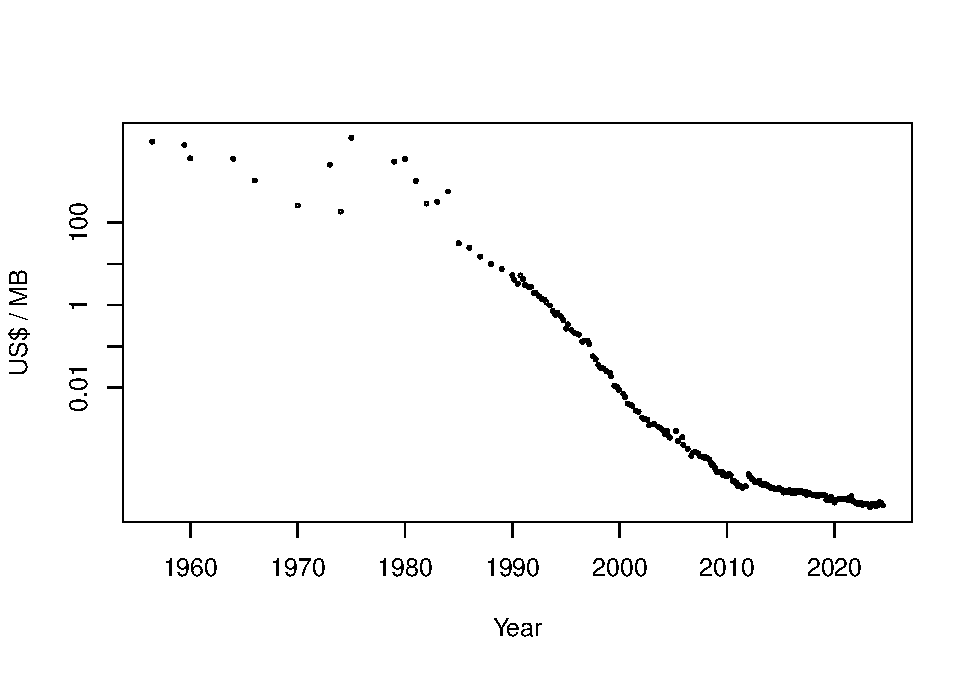
\includegraphics{_main_files/figure-latex/storage-costs-1.pdf}
\caption{\label{fig:storage-costs}The decline in storage costs per megabyte in consumer hard drives.}
\end{figure}

These technologies can potentially create vast datasets, and in order to adhere to the FAIR principles (Findable, Accessible, Interoperable, Reusable), it is important for the data to be accompanied by an appropriate suite of data standards, such as those developed by TDWG.

\section{Overall Philosophy}\label{overall-philosophy}

\subsection{Leverage what already exists}\label{leverage-what-already-exists}

Many of the tools that are needed to monitor biodiversity already exist, and the goal of WildlifeSystems is to bring these tools together in a coherent and integrated way. This will allow researchers and others to build on existing technologies to develop new tools and applications that can be used to monitor biodiversity in a wide range of environments.These tools are designed to be flexible, scalable, and easy to use, and to provide a platform for the development of new technologies and applications.

\subsection{Innovate where necessary}\label{innovate-where-necessary}

``Technology is stuff that doesn't work yet.''
\hfill --- Bran Ferren

Where suitable technological solutions already exist, use them. Limit technological research to what needs to be new. Most of the time it's OK to use existing technology, and focus development on the biodiversity related problem you're trying to solve. Older technologies are often better understood and more stable. Some of the technologies WildlifeSystems leverages to innovate in the biodiversity sphere are given in Table \ref{tab:tech-age}.

\begin{table}

\caption{\label{tab:tech-age}Age of technologies underpinning WildlifeSystems.}
\centering
\begin{tabular}[t]{l|l|l}
\hline
Technology & Year Introduced & Age in  2024\\
\hline
Ethernet & 1973 & 51\\
\hline
BASH & 1989 & 35\\
\hline
Linux & 1991 & 33\\
\hline
\end{tabular}
\end{table}

\subsection{Plan for heterogeneity}\label{plan-for-heterogeneity}

\href{https://medium.ebaker.me.uk/sensor-networks1-abstracting-heterogeneity-319c0c41c9fa}{Any network of devices will become heterogeneous given sufficient time}. The primary driver of this shift to heterogeneity is continuous technological innovation combined with obsolescence of technical components.

Secondary drivers are changes in the purpose, capabilities, and/or scale of the network over time.

The WildlifeSystems ecosystem is designed to be able to handle this heterogeneity, and to allow for the easy integration of new technologies as they become available.

\subsection{Modularise}\label{modularise}

The WildlifeSystems ecosystem is designed to be modular, with each component able to be used independently or in combination with other components. This allows users to build custom solutions that meet their specific needs, and to easily add or remove components as required.

Defined interfaces between components allow for easy integration of new technologies, and for components to be replaced or upgraded without affecting the rest of the system. This also lets contributors to focus on what they are best at.

\subsection{Open Source}\label{open-source}

\section{Structure of Wildlife Systems}\label{structure-of-wildlife-systems}

\subsection{Packages}\label{packages}

\chapter{Sensor Networks}\label{sensor-networks}

\chapter{Environmental Sensors}\label{environmental-sensors}

\section{How sensors work}\label{how-sensors-work}

\subsection{Temperature}\label{temperature}

\subsubsection{Thermistors}\label{thermistors}

A thermistor is a type of resistor whose resistance changes significantly with temperature. The word is a portmanteau of thermal and resistor.

\subsection{Humidity}\label{humidity}

\subsubsection{Capacitive Humidity Sensors}\label{capacitive-humidity-sensors}

A capacitative humidity sensor consists of a small capacitor with a hygroscopic dielectric material between two electrodes. The dielectric material, usually a plastic or polymer, has a low dielectric constant when dry. In the presence of moisture, the dielectric constant increases due to water vapor, which has a much higher dielectric constant. As moisture is absorbed, the sensor's capacitance increases. The amount of moisture absorbed depends on the surrounding temperature and water vapour pressure, which also affects the hygroscopic dielectric material used in the sensor.

\subsection{Air Pressure}\label{air-pressure}

\subsection{Gases}\label{gases}

\subsubsection{Heated Gas Resistance}\label{heated-gas-resistance}

Heated gas sensors are used to detect gases in the air. The sensor consists of a metal oxide semiconductor that is heated to a high temperature. Volatile organic compounds (VOCs) in the air change the resistance of the sensor.

These sensors are typically used indoors and have a short lifespan (perhaps two years). As such they are rarely used in environmental sensing applications, but are included on some common sensors such as the BME680.

\chapter{Sensors in WildlifeSystems}\label{sensors-in-wildlifesystems}

The WildlifeSystems platform comes with support for some popular existing environmental sensors, although there are many on the market and the range available is subject to constant change. The modular nature of WildlifeSystems allows for new sensors to be easily integrated if the need arises.

WildlifeSystems takes an abstracted approach to sensors. Interface modules are provided for each sensor, which can be used to read the sensor data into a standard format.

As many physical packages contain multiple sensors (e.g.~the supported BME680 can monitor temperature, humidity, air pressure and air quality) there is a conceptual difference between a ``device'' and the one or more sensors on a device.

\section{Devices included in the base system}\label{devices-included-in-the-base-system}

The Raspberry Pi does not come with environmental sensors, however there are several onboard sensors that are used to monitor the operation of the hardware, to prevent crucial components from overheating, including the temperature of the CPU and GPU chips. WildlifeSystems provides access to these sensors through the \texttt{sensor-onboard} package, as well as providing some \emph{software sensors} that report the free memory and free SD storage available. These can be useful for detecting and resolving possible issues on a sensor node before a serious problem arises.

\section{Installing sensor support}\label{installing-sensor-support}

Support for sensors is installed as part of the node installation process, however it is possible to install the \texttt{sensor-control} abstraction layer onto any Raspberry Pi system using the command below.

\begin{Shaded}
\begin{Highlighting}[]
\FunctionTok{wget} \AttributeTok{{-}O} \AttributeTok{{-}}\NormalTok{ https://raw.githubusercontent.com/Wildlife{-}Systems/sensor{-}control/main/install }\KeywordTok{|} \FunctionTok{sudo}\NormalTok{ bash}
\end{Highlighting}
\end{Shaded}

This will install the \texttt{sensor-control} and \texttt{sensor-onboard} scripts into the system, as well as installing a small of number of supporting packages if they are not already installed.

\section{Reading data from a device}\label{reading-data-from-a-device}

The sensor read command, \texttt{sr}, can be used to list the available devices on a given sensor.

\begin{Shaded}
\begin{Highlighting}[]
\ExtensionTok{sr}\NormalTok{ onboard list}
\end{Highlighting}
\end{Shaded}

The sensor read command, \texttt{sr}, can also be used to read data from a named sensor. Not specifying a sensor is equivalent to reading all sensors on that device (i.e.~using the wildcard''*``).

\begin{Shaded}
\begin{Highlighting}[]
\ExtensionTok{sr}\NormalTok{ onboard}
\ExtensionTok{sr}\NormalTok{ onboard }\PreprocessorTok{*}
\ExtensionTok{sr}\NormalTok{ onboard onboard\_gpu}
\end{Highlighting}
\end{Shaded}

This will give a JSON string listing information about each sensor (or just the specified sensor), and the current reading. This information can be presented in a more human readable form by piping the output to the program \texttt{jq}, a command line JSON processor.

\begin{Shaded}
\begin{Highlighting}[]
\ExtensionTok{sr}\NormalTok{ onboard }\KeywordTok{|} \ExtensionTok{jq}
\end{Highlighting}
\end{Shaded}

\section{The sensor reading process}\label{the-sensor-reading-process}

The sensor reading process in WildlifeSystems has five steps.

\begin{enumerate}
\def\labelenumi{\arabic{enumi}.}
\item
  The \texttt{sr} command identifies which device script to route the request to.
\item
  The sensor script calls the \texttt{sc-prototype} script to obtain a template (``prototype'') of the JSON request.
\item
  The sensor script accesses the relevant sensor(s) and populates the values in a template for each sensor reading, before returning a JSON array of populated readings to \texttt{sr}.
\item
  The \texttt{sr} script populates additional information for each reading, providing the \texttt{node\_id} and a \texttt{timestamp} for each.
\item
  \texttt{sr} returns the finalised JSON array to the user.
\end{enumerate}

\section{Installing new sensors}\label{installing-new-sensors}

\chapter{Supported sensors}\label{supported-sensors}

\section{DHT11}\label{dht11}

The DHT11 is a low-cost temperature and humidity sensor. It uses a capacitive humidity sensor and a thermistor to measure the surrounding air, and sends the data by digital signals on the data pin.

The low-cost nature of the sensor makes it useful desp ite several shortcomings, e.g.~for monitoring the temperature and humidity inside electronics enclosures where accuracy is not critical but the sensor can provide critical early warning of overheating or condensation.

\section{BME680}\label{bme680}

4-in-1 sensor that provides humidity, temperature, pressure, and gas readings.

\chapter{Implementing new sensors}\label{implementing-new-sensors}

New sensors should be implemented as new packages (i.e, a new GitHub repository). Packages have a standard format, and should be named \texttt{sensor-\textless{}sensor-name\textgreater{}} where \texttt{\textless{}sensor-name\textgreater{}} is short, descriptive of the sensor (e.g.~model number), and unique within the WildlifeSystems ecosystem.

The structure of a basic package is given below.

\begin{verbatim}
.
+-- inst
|   +-- files that are not part of the package structure
|       used during installation (e.g. 3rd party scripts 
|       to be copied to /usr/bin/)
|
+-- sensor-<sensor-name>
|     Executable to read sensor and print JSON of readings
|     (copied on install to /usr/bin/)
|
+-- <sensor-name>
|     Configuration file 
|     (copied on install to /var/aao/sensors/)
|
+-- install
|     Bash file run once on install - used to install packaged
|     dependencies, etc.
\end{verbatim}

As many people implement various sensors on the Raspberry Pi, it is likely that some sort of solution is already available, that can be tweaked to output readings in the standard format required. However, you must ensure that any licensing conditions are met. In particular, an open license is required if submitting your sensor package to WildlifeSystems for inclusion in the ecosystem.

\section{Reading the sensor}\label{reading-the-sensor}

File \texttt{sensor-\textless{}sensor-name\textgreater{}} provides the functionality to read the protoype JSON, populate the JSON with sensor readings, and print the output.

The file can be written in any programming or scripting language, but to prevent overhead consideration should be given to minimising the number of new packages installed.

\subsection{In bash}\label{in-bash}

\begin{Shaded}
\begin{Highlighting}[]
\CommentTok{\#!/bin/bash}

\CommentTok{\# Read the prototype JSON}
\VariableTok{JSON}\OperatorTok{=}\VariableTok{$(}\ExtensionTok{sc{-}prototype}\VariableTok{)}

\BuiltInTok{echo} \AttributeTok{{-}n} \StringTok{"["}

\CommentTok{\# Code to read the sensor value into GPU\_TEMP}

\CommentTok{\# Use \textasciigrave{}jq\textasciigrave{} to modify JSON}
\VariableTok{SENSOR}\OperatorTok{=}\VariableTok{$(}\BuiltInTok{echo} \VariableTok{$JSON} \KeywordTok{|} \ExtensionTok{jq} \StringTok{".sensor |= }\DataTypeTok{\textbackslash{}"}\StringTok{onboard\_gpu}\DataTypeTok{\textbackslash{}"}\StringTok{ | .measures |= }\DataTypeTok{\textbackslash{}"}\StringTok{temperature}\DataTypeTok{\textbackslash{}"}\StringTok{ | .unit |= }\DataTypeTok{\textbackslash{}"}\StringTok{Celsius}\DataTypeTok{\textbackslash{}"}\StringTok{| .value |= }\VariableTok{$\{GPU\_TEMP\}}\StringTok{"}\VariableTok{)}
\BuiltInTok{echo} \AttributeTok{{-}n} \VariableTok{$SENSOR}

\BuiltInTok{echo} \StringTok{"]"}
\end{Highlighting}
\end{Shaded}

\subsection{In Python}\label{in-python}

\begin{Shaded}
\begin{Highlighting}[]
\CommentTok{\#!/}
\ImportTok{import}\NormalTok{ os}
\ImportTok{import}\NormalTok{ json}

\CommentTok{\# Read the prototype JSON}
\NormalTok{stream }\OperatorTok{=}\NormalTok{ os.popen(}\StringTok{\textquotesingle{}sc{-}prototype\textquotesingle{}}\NormalTok{)}
\NormalTok{output }\OperatorTok{=}\NormalTok{ stream.read()}

\CommentTok{\# Pre{-}populate with sensor metadata}
\NormalTok{temperature }\OperatorTok{=}\NormalTok{ json.loads(output)}
\NormalTok{temperature[}\StringTok{"sensor"}\NormalTok{] }\OperatorTok{=} \StringTok{"bme680\_temperature"}
\NormalTok{temperature[}\StringTok{"measures"}\NormalTok{] }\OperatorTok{=} \StringTok{"temperature"}
\NormalTok{temperature[}\StringTok{"unit"}\NormalTok{] }\OperatorTok{=} \StringTok{"Celsius"}

\CommentTok{\# Code to read sensor and output in variable \textasciigrave{}sensor\_reading\textasciigrave{}}
\NormalTok{temperature[}\StringTok{"value"}\NormalTok{] }\OperatorTok{=}\NormalTok{ sensor\_reading}

\CommentTok{\# Output the JSON in an array}
\BuiltInTok{print}\NormalTok{(}\StringTok{"["}\NormalTok{,json.dumps(temperature),}\StringTok{"]"}\NormalTok{)}
\end{Highlighting}
\end{Shaded}

\section{Setting the environment}\label{setting-the-environment}

The file \texttt{\textless{}sensor-name\textgreater{}} in the package specifies information that modify the environment of the Raspberry Pi (e.g.~if the i2c interface should be enabled) before the \texttt{sensor-\textless{}sensor-name\textgreater{}} script is run. This allows sensors with different requirements to run sequentially on the same node.

The file must always be present, even if it is empty. During installation the file is moved to \texttt{/var/aao/sensors/} and the list of files in this directory indicates to the system which sensors are installed.

TODO: i2c

\section{Install}\label{install}

The file \texttt{install} in the directory is run once, when the sensor package is installed. This allows for the installation of packages and scripts necessary for the functioning of the package.

The file is executed by \texttt{bash} and the use of \texttt{sudo} is allowed.

\section{\texorpdfstring{The installation process with \texttt{si}}{The installation process with si}}\label{the-installation-process-with-si}

The sensor install script, \texttt{si}, from \texttt{sensor-control} is used to install sensor packages. For developer reference the installation process is described below.

\begin{enumerate}
\def\labelenumi{\arabic{enumi}.}
\item
  \texttt{si} clones the \texttt{Wildlife-Systems/sensor-\textless{}sensor-name\textgreater{}} repository from GitHub.
\item
  The \texttt{install} script is executed.
\item
  \texttt{sensor-\textless{}sensor-name} is marked as executable and move to /usr/bin/.
\item
  \texttt{\textless{}sensor-name\textgreater{}} is moved to /var/aao/sensors/.
\item
  The cloned repository is removed from the local filesystem.
\end{enumerate}

\section{Submitting packages to WildlifeSystems}\label{submitting-packages-to-wildlifesystems}

Submitting packages (where licensing allows) to WildlifeSystems allows the ecosystem to be developed and sustained collaboratively by the user community.

Packages can be sent to the administrators as a compressed file, or a request can be sent to fork an existing GitHub repository. Contact details can be found at \url{https://wildlife.systems/contact.html}.

\chapter{Sound Devices}\label{sound-devices}

\section{How sound devices work}\label{how-sound-devices-work}

\chapter{Sound devices in WildlifeSystems}\label{sound-devices-in-wildlifesystems}

\chapter{Imaging Devices}\label{imaging-devices}

\section{How imaging devices work}\label{how-imaging-devices-work}

\chapter{Imaging devices in WildlifeSystems}\label{imaging-devices-in-wildlifesystems}

\chapter{Power Management}\label{power-management}

Power management on the Raspberry Pi is useful when deployments are made that are powered by batteries and/or renewable sources such as solar power that are intermittent.

In addition, there are small environmental benefits on consuming less power on systems which have continual grid power.

The \texttt{pi-pwr} script can be used to turn off unused functionality, either always or just when it is not required.

\section{Installation of power management tools}\label{installation-of-power-management-tools}

The power management tools are installed as part of the node installation process, however they can be easily installed independently on any Raspberry Pi system.

\begin{Shaded}
\begin{Highlighting}[]
\FunctionTok{wget} \AttributeTok{{-}O} \AttributeTok{{-}}\NormalTok{ https://github.com/wildlife{-}systems/pi{-}pwr/raw/master/install }\KeywordTok{|} \FunctionTok{sudo}\NormalTok{ bash}
\end{Highlighting}
\end{Shaded}

\section{Turning funtionality on and off}\label{turning-funtionality-on-and-off}

\section{Considerations}\label{considerations}

Disabling all network functionality will prevent the node from communicating until either the functionality is turned back on or the Raspberry Pi is restarted.

If disabling all connectivity is desired periodically then the functionality to turn these systems back on must be scripted.

\subsection{\texorpdfstring{A note on \texttt{sudo}}{A note on sudo}}\label{a-note-on-sudo}

Raspberry Pi OS (and previously Raspbian) allows the default user to run sudo without a password. This is not true for other Linux distributions, such as Ubuntu. This could lead to a password prompt when using \texttt{pi-pwr}. As nodes are designed to run autonomously, the installation process for \texttt{ws-node} will configure \texttt{pi-pwr} to not require a \texttt{sudo} password.

\chapter{Indicators and heartbeats}\label{indicators-and-heartbeats}

The script \texttt{ws-indicate} is used to indicate the device's status using the LED(s) on board the Raspberry Pi. The script \texttt{ws-heartbeat} can be used to transmit the device's status to a user-defined script that could provide logging, or submit the status to an online dashboard.

\section{\texorpdfstring{Installation of \texttt{ws-indcate} and \texttt{ws-heartbeat}}{Installation of ws-indcate and ws-heartbeat}}\label{installation-of-ws-indcate-and-ws-heartbeat}

These tools are installed as part of the node installation process.

\section{Indicators}\label{indicators}

Internally \texttt{ws-inidicate} makes repeated calls to \texttt{pi-pwr} to control the LED(s). There are three indicator routines, heartbeat (quick flash of LEDs in order to show device is functioning), countdown (flashes power LED), and record (power LED on, action LED off).

\begin{Shaded}
\begin{Highlighting}[]
\FunctionTok{sudo}\NormalTok{ ws{-}indicate}
\FunctionTok{sudo}\NormalTok{ ws{-}indicate countdown 5   }\CommentTok{\# counts down from 5}
\FunctionTok{sudo}\NormalTok{ ws{-}indicate record action }\CommentTok{\# record light is on while action is executed}
\end{Highlighting}
\end{Shaded}

\subsection{\texorpdfstring{A note on \texttt{sudo}}{A note on sudo}}\label{a-note-on-sudo-1}

Raspberry Pi OS (and previously Raspbian) allows the default user to run sudo without a password. This is not true for other Linux distributions, such as Ubuntu. This could lead to a password prompt when using \texttt{ws-indicate}. As nodes are designed to run autonomously, the installation process for \texttt{ws-node} will configure \texttt{ws-indicate} to not require a \texttt{sudo} password.

\section{Heartbeat}\label{heartbeat}

The script \texttt{ws-heartbeat} is used to send a heartbeat signal to the devices.wildlife.systems server to indicate that the node is alive and connected, as well as to provide some information to assist problem diagnosis. The data sent comes from the onboard sensor readings (\texttt{sr\ onboard}) and the server stores the node ID, timestamp, CPU and GPU temperatures, and the amount of memory and storage used. The node must be registered with WildlifeSystems for this data to be stored.

The script may be run for debugging purposes at any time as follows.

\begin{Shaded}
\begin{Highlighting}[]
\ExtensionTok{ws{-}heartbeat}
\end{Highlighting}
\end{Shaded}

The script will exit silently on success.

\chapter{Integration with monitoring tools}\label{integration-with-monitoring-tools}

\section{PRTG}\label{prtg}

As the devices are Raspberry Pi based, we can use the PRTG monitoring tool to monitor standard aspects of their performance including CPU, memory, disk space, and network traffic.

\subsection{Monitoring custom sensors}\label{monitoring-custom-sensors}

Some sensors attached to WildlifeSystems nodes may be used to monitor aspects of the devices themselves, rather than the environment. Using custom PRTG scripts it is possible to include these measurements in PRTG reports and alerts.

The following example reports the humidity of the device enclosure measured by a DHT11 sensor. It makes use of the WildlifeSystems \texttt{sr} command to read the sensor in a standard JSON format, and converts the reading to a format expected by PRTG.

\begin{Shaded}
\begin{Highlighting}[]
\CommentTok{\#!/bin/bash}

\VariableTok{HV}\OperatorTok{=}\VariableTok{$(}\FunctionTok{sudo}\NormalTok{ sr dht11 }\KeywordTok{|} \ExtensionTok{jq} \StringTok{\textquotesingle{}map(select(.sensor == "dht11\_humidity")) | .[]["value"]\textquotesingle{}}\VariableTok{)}

\ControlFlowTok{if} \KeywordTok{((} \VariableTok{$HV} \OperatorTok{\textless{}} \DecValTok{75} \KeywordTok{));} \ControlFlowTok{then}
  \ExtensionTok{/bin/echo} \StringTok{"0:}\VariableTok{$HV}\StringTok{:Acceptable humidity"}
\ControlFlowTok{else}
  \ExtensionTok{/bin/echo} \StringTok{"4:}\VariableTok{$HV}\StringTok{:Too humid"}
\ControlFlowTok{fi}
\end{Highlighting}
\end{Shaded}

\chapter{Developer Guidelines}\label{developer-guidelines}

\section{Documentation}\label{documentation}

There are three main kinds of documentation in the WildlifeSystems project.

\begin{enumerate}
\def\labelenumi{\arabic{enumi}.}
\item
  \textbf{Code comments}: Primarily for future you (or someone similar) to get to grips with your code. \emph{Why does this code do this?}.
\item
  \textbf{Package documentation}: Describes what your package does, how it interacts with the larger system. \emph{What will this package do for me?}
\item
  \textbf{Overall project documentation}: This manual. \emph{How do I use the entire system for my research?}
\end{enumerate}

\chapter{Server Tools}\label{server-tools}

These tools are only needed for running and maintaining the \href{https://wildlife.systems}{wildlife.systems} webserver.

\section{Installation}\label{installation}

\begin{Shaded}
\begin{Highlighting}[]
\FunctionTok{git}\NormalTok{ clone git@github.com:Wildlife{-}Systems/wildlife.systems{-}tools.git}
\BuiltInTok{cd}\NormalTok{ wildlife.systems{-}tools}
\ExtensionTok{./install}
\FunctionTok{cp}\NormalTok{ .ws{-}db.php \textasciitilde{}/}

\CommentTok{\#Edit \textasciitilde{}/.ws{-}db.php to connect to the wildlife{-}systems database}
\end{Highlighting}
\end{Shaded}

\section{Adding nodes and receieving a token}\label{adding-nodes-and-receieving-a-token}

\begin{Shaded}
\begin{Highlighting}[]
\ExtensionTok{ws{-}node{-}add} \OperatorTok{\textless{}}\NormalTok{node\_id}\OperatorTok{\textgreater{}}
\end{Highlighting}
\end{Shaded}

Adding a node by it's ID (serial number of the Raspberry Pi) will add the device to the wildlife.systems database, generate a token, and display the token (a UUID) in the console. This token is used to authenticate the device when it sends data to wildlife.systems.

\section{Removing a node}\label{removing-a-node}

\begin{Shaded}
\begin{Highlighting}[]
\ExtensionTok{ws{-}node{-}remove} \OperatorTok{\textless{}}\NormalTok{node\_id}\OperatorTok{\textgreater{}}
\end{Highlighting}
\end{Shaded}

\appendix


\chapter{Return codes}\label{return-codes}

The various scripts that form the WildlifeSystems ecosystem use a standard set of return codes.

\section{00-09 Script functionality}\label{script-functionality}

\begin{tabular}{l|l|l}
\hline
Code & Label & Description\\
\hline
0 & OK & Terminated normally. No error.\\
\hline
1 & Already running & The script determined it was already running and terminated.\\
\hline
2 & No arguments & The script requires arguments but none given. Will give help text.\\
\hline
\end{tabular}

\section{10-19 Parameter problems}\label{parameter-problems}

\begin{tabular}{l|l|l}
\hline
Code & Label & Description\\
\hline
10 & Invalid argument & One or more of the arguments to the script was invalid.\\
\hline
11 & Incorrect filename pattern & A standard filename pattern was expected. Allowed values are 'timestamp'.\\
\hline
\end{tabular}

\section{20-29 Sensor problems}\label{sensor-problems}

\begin{tabular}{l|l|l}
\hline
Code & Label & Description\\
\hline
20 & Unknown device & This device is not supported, or software is not installed.\\
\hline
21 & Unknown sensor & This sensor is not known on this device.\\
\hline
\end{tabular}

\section{30-39 Sound device problems}\label{sound-device-problems}

\begin{tabular}{l|l|l}
\hline
Code & Label & Description\\
\hline
30 & Unsupported device & The specified device is unsupported.\\
\hline
31 & Unsupported feature & This feature is not present on the sound device.\\
\hline
32 & Unknown feature & The feature requested is unknown.\\
\hline
\end{tabular}

\section{40-49 Image device problems}\label{image-device-problems}

\begin{tabular}{l|l|l}
\hline
Code & Label & Description\\
\hline
40 & Unsupported device & The specified device is unsupported.\\
\hline
41 & Unsupported feature & This feature is not present on the sound device.\\
\hline
42 & Unknown feature & The feature requested is unknown.\\
\hline
\end{tabular}

\section{50-59 Power management problems}\label{power-management-problems}

\begin{tabular}{l|l|l}
\hline
Code & Label & Description\\
\hline
50 & Disallowed value (should be on or off) & The specified device is unsupported.\\
\hline
51 & Disallowed value (should be on, off or default) & This feature is not present on the sound device.\\
\hline
\end{tabular}

\section{60-69 Special meanings}\label{special-meanings}

\begin{tabular}{l|l|l}
\hline
Code & Label & Description\\
\hline
60 & Identify as a sensor device script & Returned by sensor device script in response to first parameter `identify`.\\
\hline
\end{tabular}

  \bibliography{book.bib,packages.bib}

\end{document}
